%! Author = user
%! Date = 25/01/2021

% Preamble
\documentclass[11pt]{article}

\begin{document}

    \subsection{The Adapter Pattern}
    The pattern coverts the interface of a class into another interface that clients expect. It allows classes to work together
    that couldn't otherwise because of incompatible interfaces.
    \begin{itemize}
        \item Client (Duck Simulator) is composed with the class with the Target interface.
        \item Adapter (TurkeyAdapter) is composed with the adaptee (Turkey) and delegates calls to the adaptee, and
        returns any needed value.
        \item The Client (Duck Simulator) and the adaptee (Turkey) don't know there's an adapter (TurkeyAdapter) in between.\\
        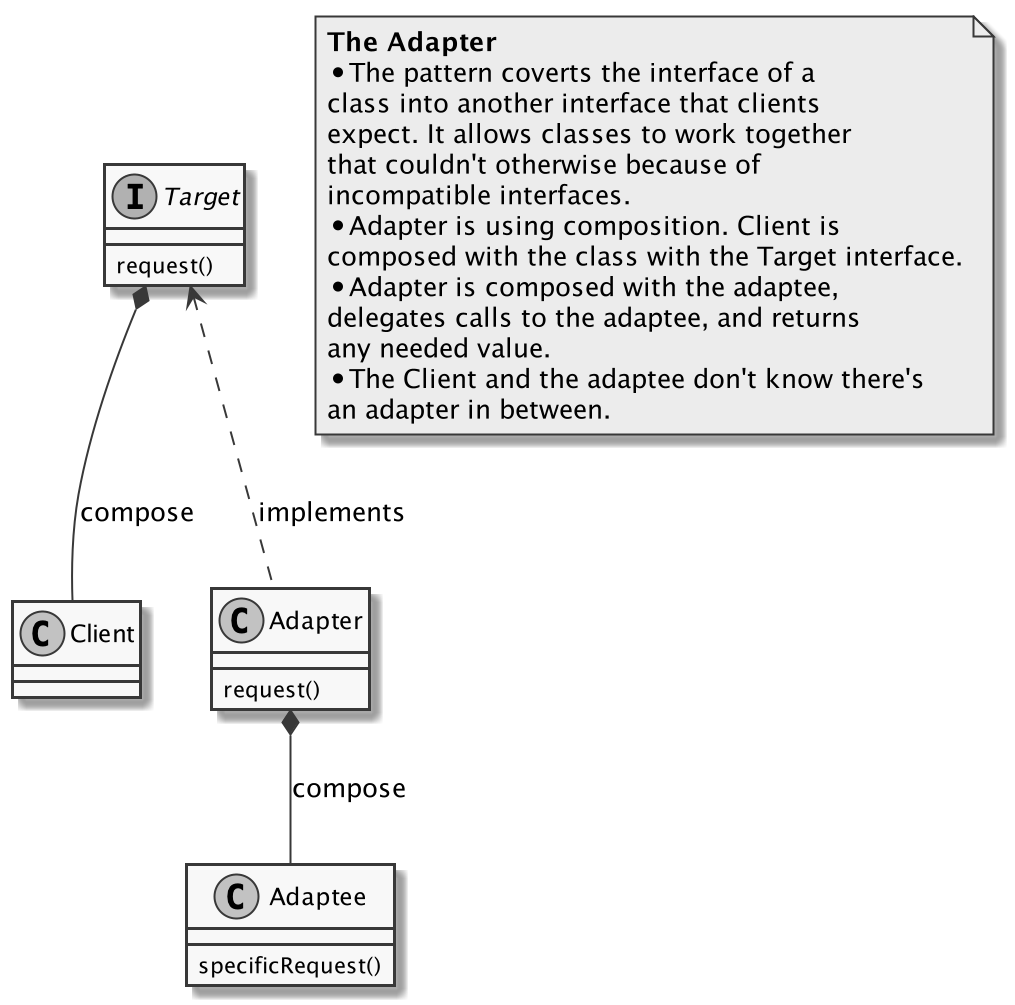
\includegraphics[scale=0.15]{adapter/1_adapter_pattern}
        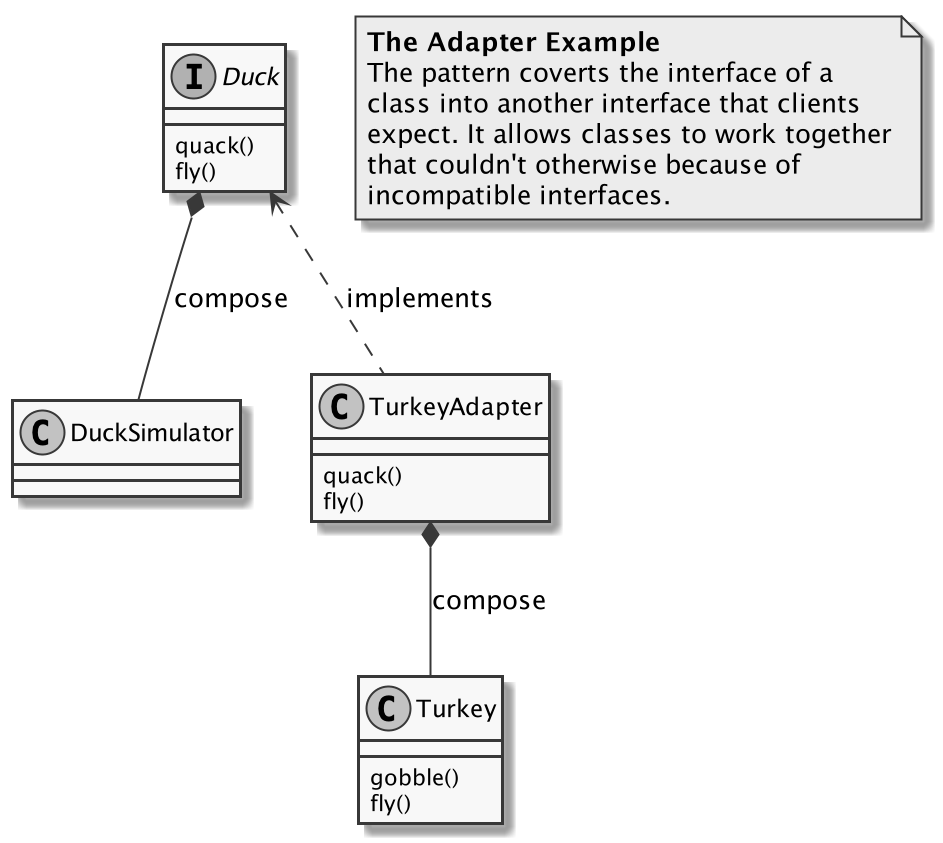
\includegraphics[scale=0.15]{adapter/2_turkey_duck_adapter}
        \item C++ code:
        \begin{multicols}{2}
            \begin{lstlisting}
class Duck {
public:
    virtual void fly() const = 0;
    virtual void quack() const = 0;
};

class MallardDuck : public Duck{
public:
    MallardDuck(){}

    void fly() const override {
       std::cout << "fly" << std::endl;
    };
    void quack() const override {
        std::cout << "quack" << std::endl;
    };
};

// this is the client
class DuckSimulator {
public:
    void TestDuck(const Duck& duck) {
        duck.fly();
        duck.quack();
    }
};

TEST(adapter, duck) {
    DuckSimulator ds;
    MallardDuck mallardDuck;
    ds.TestDuck(mallardDuck);
}

class Turkey {
public:
     virtual void gobble() = 0;
     virtual void fly() = 0;
};

class WildTurkey : public Turkey {
    void gobble() {
        std::cout << "gobble" << std::endl;
    }
    void fly() {
        std::cout << "fly" << std::endl;
    }
};

// we can't use turkeys in the duck simulator because it expects a duck interface.
// we need to create an adapter.
class TurkeyAdapter : public Duck {
public:
    TurkeyAdapter(std::shared_ptr<Turkey> turkey) :
        turkey_(turkey){};
    void fly() const override{
        turkey_->gobble();
    };
    void quack() const override {
        turkey_->fly();
    };
private:
    std::shared_ptr<Turkey> turkey_;
};

TEST(adapter, turkey_duck_adapter) {
    DuckSimulator ds;
    MallardDuck mallardDuck;
    ds.TestDuck(mallardDuck);

    auto wildTurkey = std::make_shared<WildTurkey>();
    TurkeyAdapter turkeyAdapter(wildTurkey);
    ds.TestDuck(turkeyAdapter);
}
            \end{lstlisting}
        \end{multicols}
    \end{itemize}

    \subsection{The Bridge Pattern}
    ....
    \begin{itemize}
        \item ....
    \end{itemize}

    \subsection{The Composite Pattern}
    The Coposite Pattern allows you to compose objects into tree structures to represent part-whole hierarchies. Composite
    lets clients treat individual objects and compositions of objects uniformly.
    \begin{itemize}
        \item Using a composite structure, we can apply tha same operations over both composites and individual objects.
        In other words, in most cases we can ignore the differences between compositions of objects and individual objects.\\
        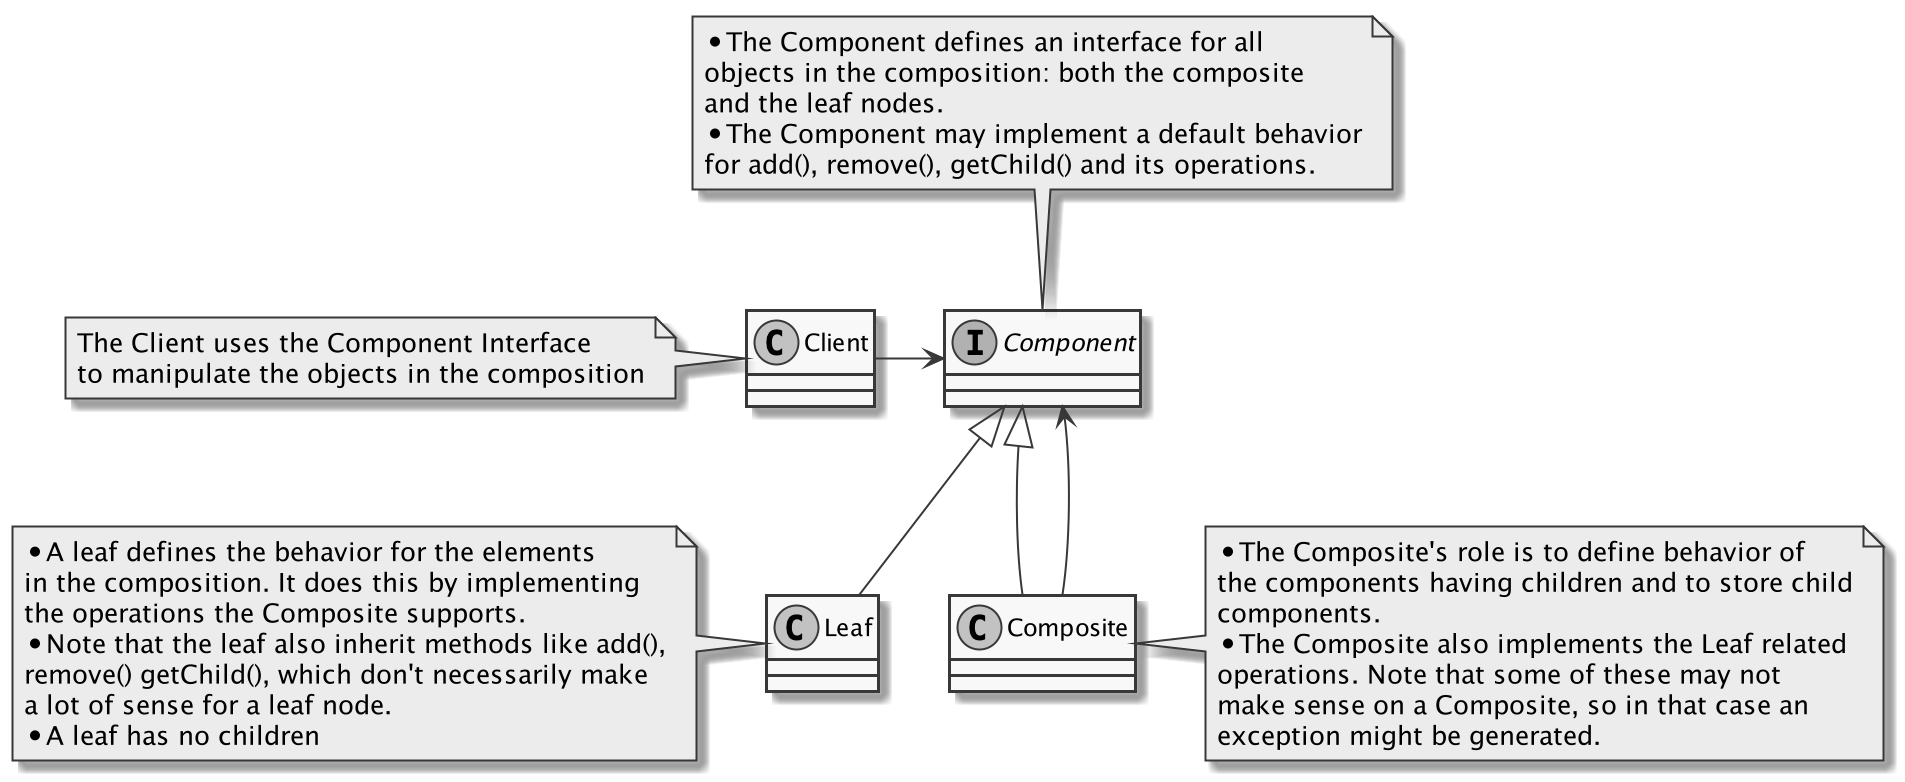
\includegraphics[scale=0.15]{composite/1__composite_pattern}
        \item Image a graphical user interface; there you'll oftern find a top level component like a Frame of Panel, containing
        other components, like menus, text, panes, scrollbars and buttons. So you GUI consist of sevaral parts, but when you display
        it, you generally think of it as a whole. You tell the top level component to display, and count on that component to
        display all its parts. We call the compnents that contain other components, "compopsite objects", and components that
        don't contain other components, "leaf objects".
        \begin{multicols}{2}
            \begin{lstlisting}
struct GraphicsObject {
    virtual void draw() = 0;
};

struct MyCircle : GraphicsObject {
    void draw() override {
        std::cout<< "Cirlce" << std::endl;
    }
};

struct Group : GraphicsObject {
    std::string name_;
    std::vector<GraphicsObject*> objects_;

    Group(const std::string& name) : name_{name} {
    }

    void draw() override {
       std::cout << "Group " << name_ << " contains: " << std::endl;
       for (auto&& o : objects_) {
           o->draw();
       }
    }
};

TEST(composite, geometric_shapes) {
    MyCircle c1, c2, c3, c4;

    Group root("root");
    root.objects_.push_back(&c1);

    Group subgroup("sub");
    subgroup.objects_.push_back(&c2);
    root.objects_.push_back(&subgroup);

    Group subsubgroup("subsub");
    subsubgroup.objects_.push_back(&c3);
    subsubgroup.objects_.push_back(&c4);
    subgroup.objects_.push_back(&subsubgroup);

    root.draw();
    // this draws all the graphical objects in the "tree", from the root down.
    // we have a uniform interface that treat
    // both singular objects as groups in a uniform manner.
}
            \end{lstlisting}
        \end{multicols}
        \item The clients don't have to worry about whether they're dealing with a composite object or a leaf object. so they dont
        have to write if statements everywhere to make sure they're calling the right methods on the right objects. Often, they
        can make one method call and execute an operation over an entire structure.
    \end{itemize}

    \subsection{The Decorator Pattern}
    This pattern attaches additional responsibilities to an object dynamically. Decorators provide a flexible alternative to
    subclassing for extending functionality.
    \begin{itemize}
        \item Here we compare two "beverages and condiments" designs using inheritance and composition.\\
        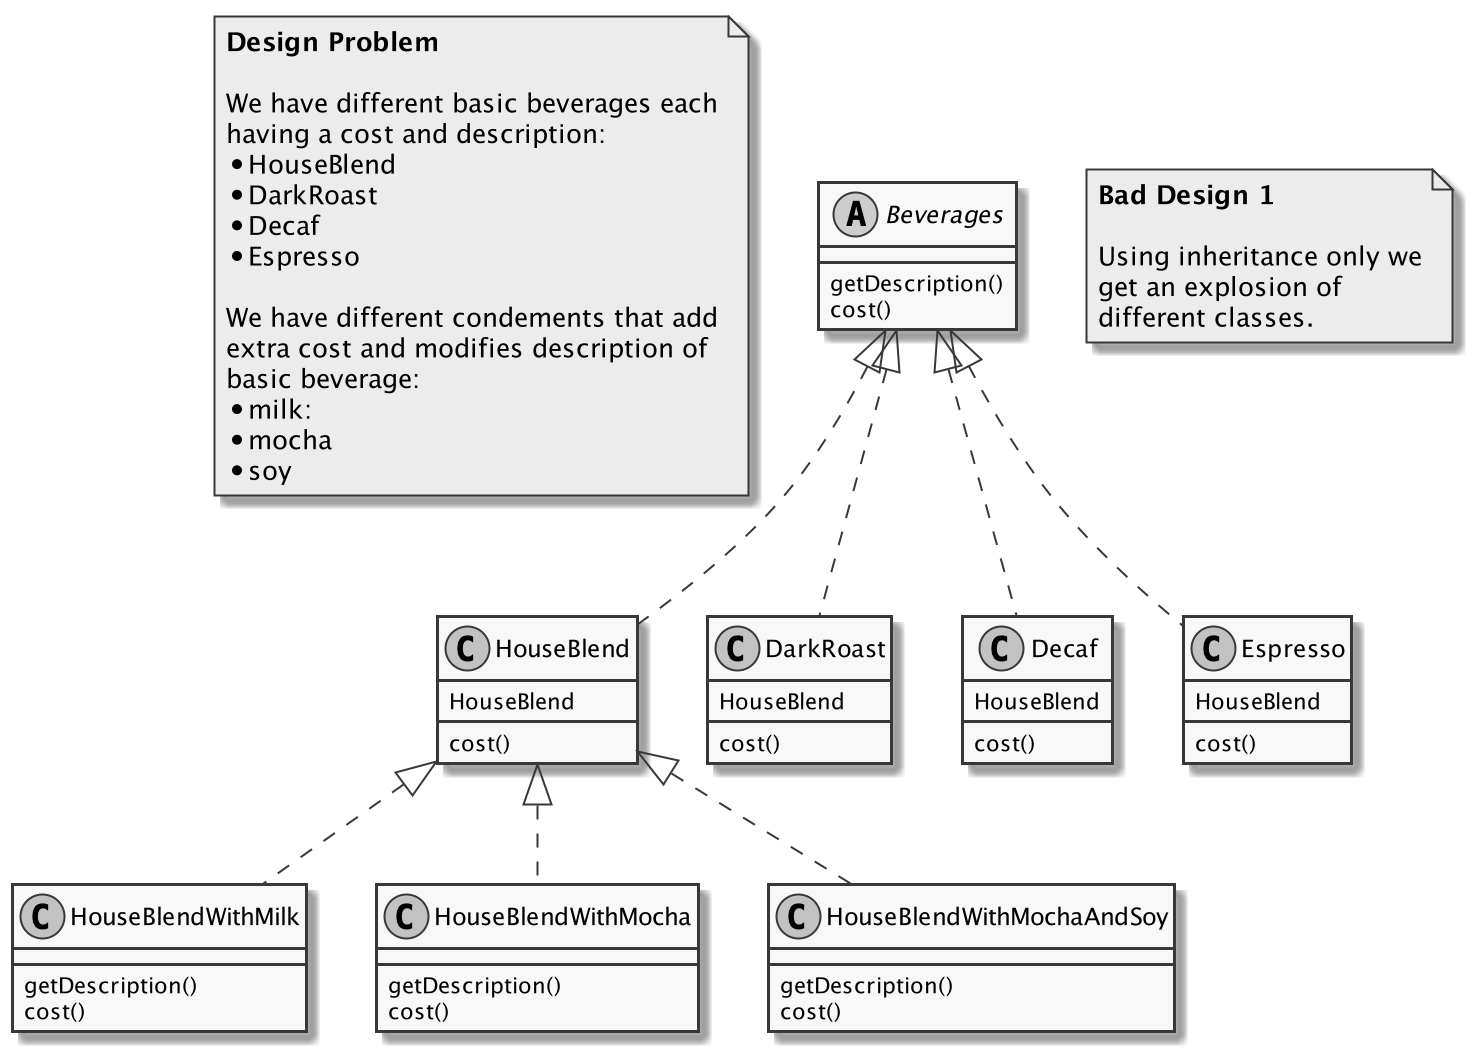
\includegraphics[scale=0.15]{decorator/1__beverages_bad_design1.png}\\
        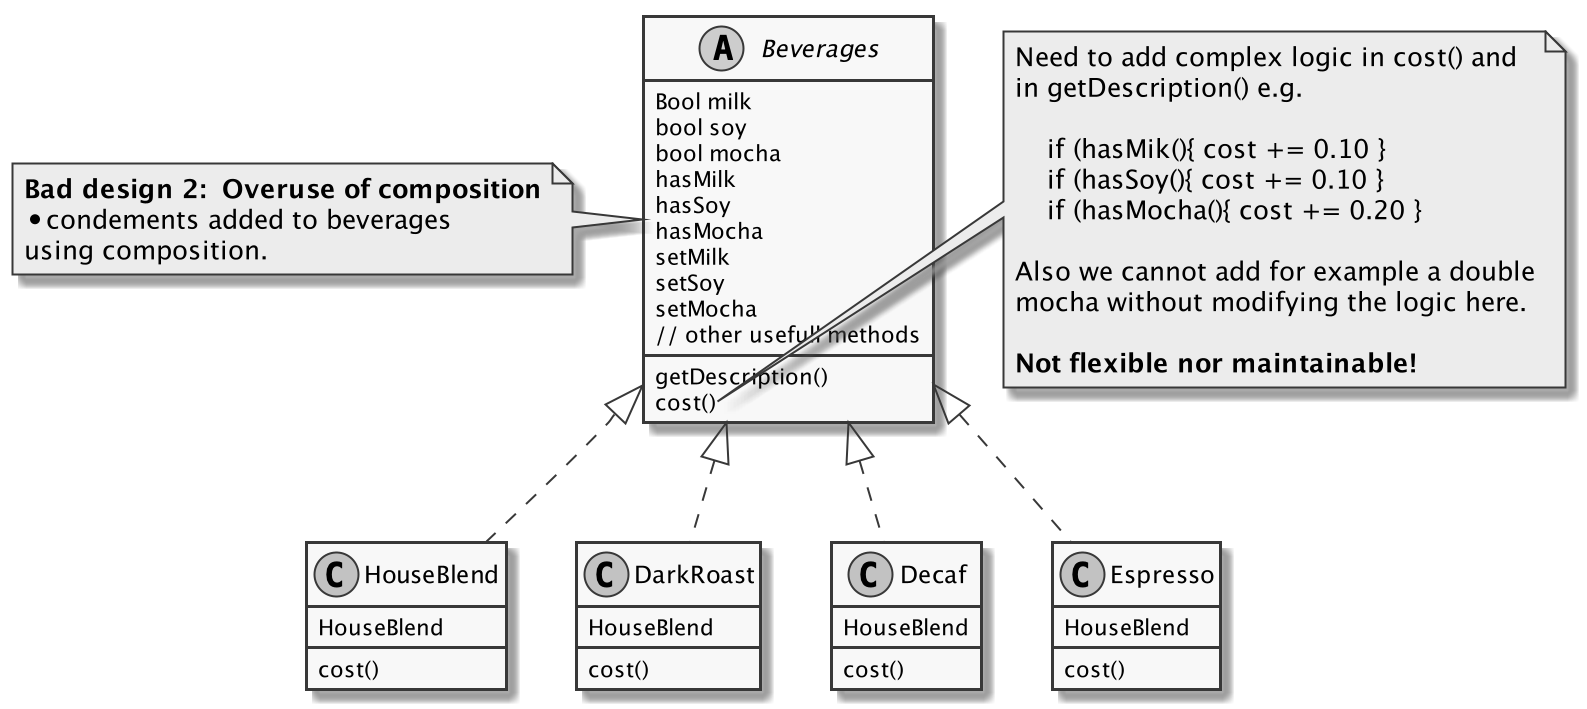
\includegraphics[scale=0.15]{decorator/2__beverages_bad_design2.png}
        \item Using exesive use of inheritance or composition can lead to unflexible and unmaintainable designs.
        \item Making use of the decorator pattern we can add additional responsibilities to an object dynamically. Making full
        use of the open-close principle.
        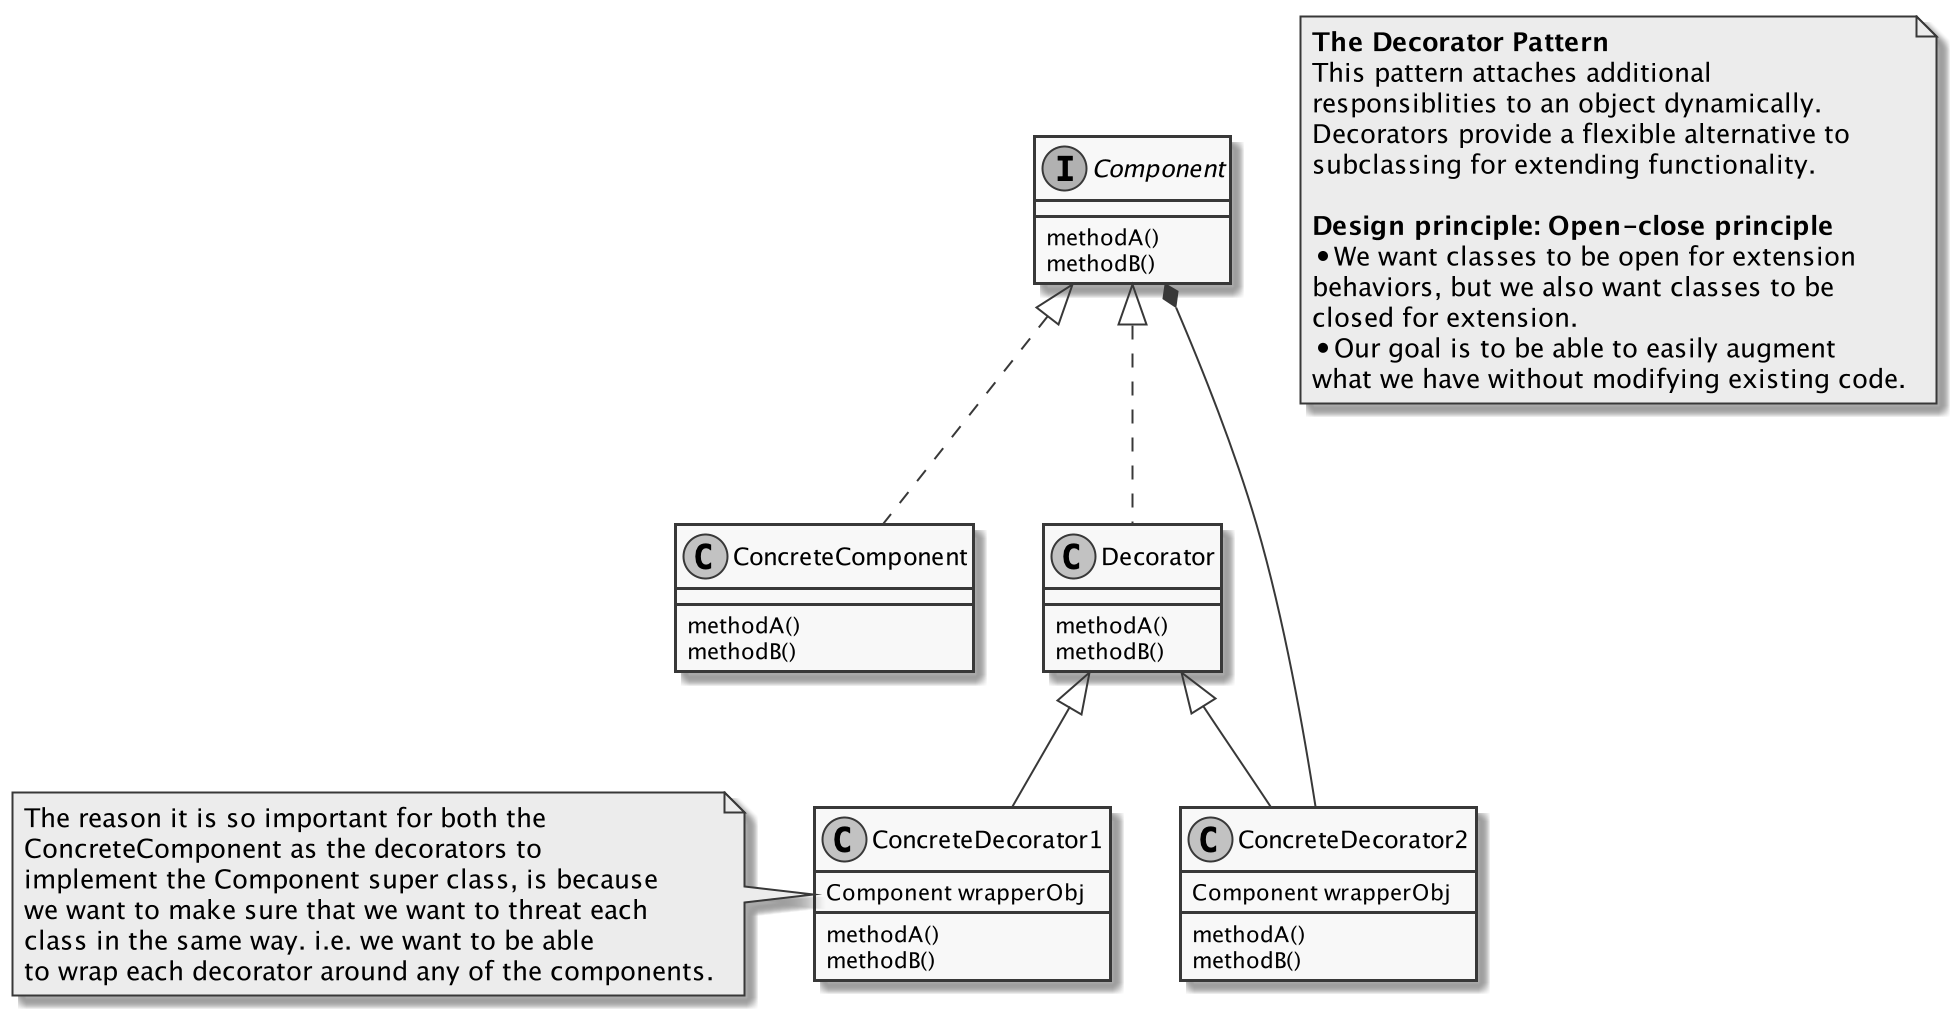
\includegraphics[scale=0.15]{decorator/3__decorator.png}
        \item The Decorator pattern applied to the beverage design:\\
        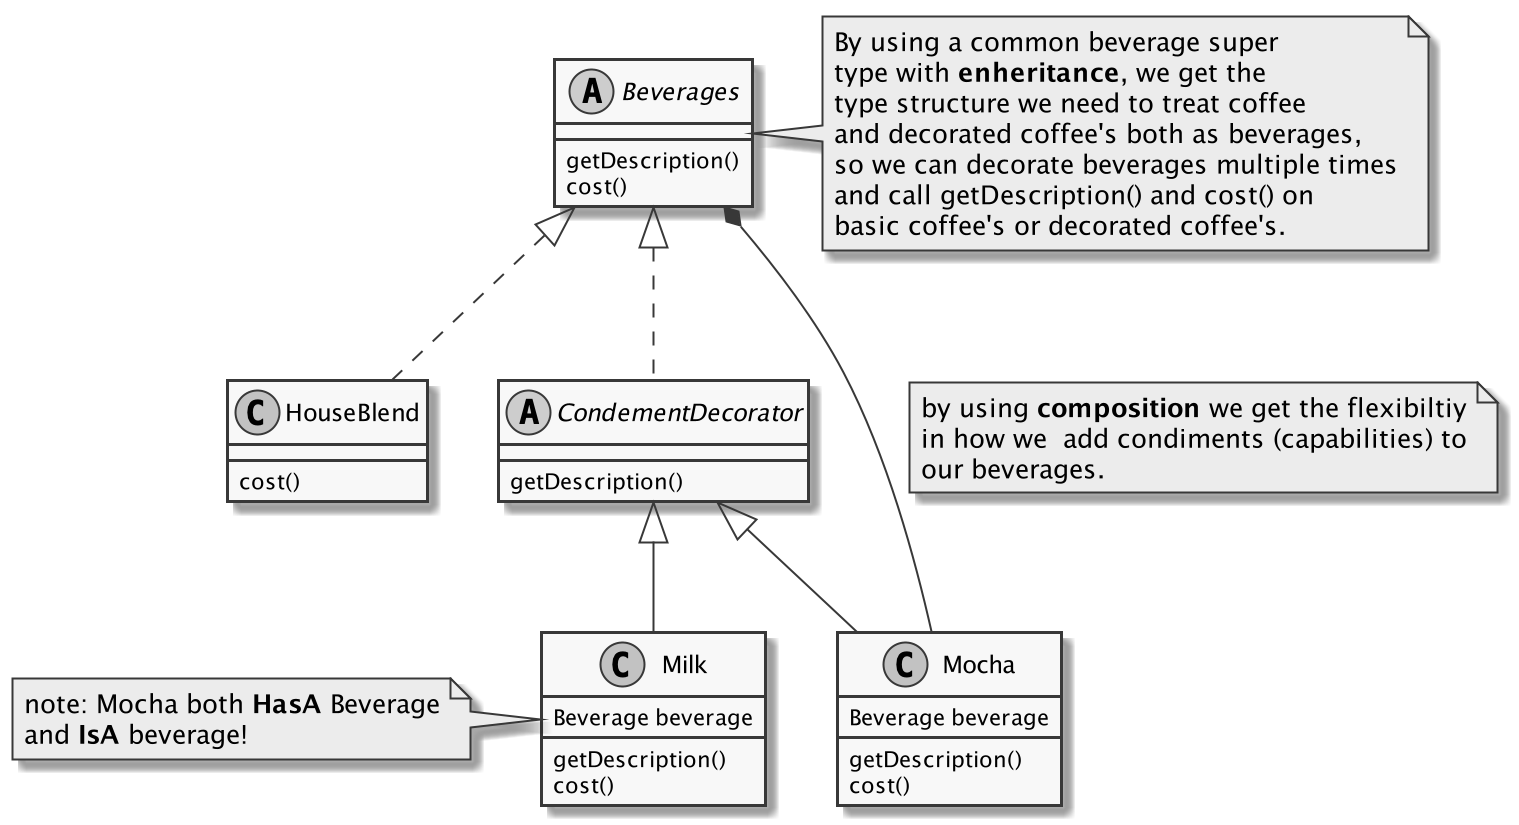
\includegraphics[scale=0.15]{decorator/4__beverages.png}
        \item C++ code:
        \begin{multicols}{2}
            \begin{lstlisting}
class Beverage {
protected:
    std::string description_ = "Unknown Beverage";
public:
    virtual std::string getDescription() {
        return description_;
    }
    virtual double cost() = 0;
};

class DarkRoast : public Beverage {
public:
    DarkRoast(){
        description_ = "Dark Roast Coffee";
    }
    double cost() {
        return 0.99;
    }
};

class CondimentDecorator : public Beverage {
    virtual std::string getDescription() = 0;
    virtual double cost() = 0;
};

class Whip : public CondimentDecorator {
private:
    std::shared_ptr<Beverage> beverage_;
public:
    Whip (std::shared_ptr<Beverage> beverage): beverage_(beverage) {
    }
    std::string getDescription() {
        return beverage_->getDescription() + ", Whip";
    };
    double cost() {
        return beverage_->cost() + 0.10;
    };
};

TEST(decorator, StarBuzzCoffee) {
    std::shared_ptr<Beverage> beverage = std::make_shared<DarkRoast>();
    std::cout << beverage->getDescription() << std::endl;
    std::cout << beverage->cost() << std::endl;

    beverage = std::make_shared<Whip>(beverage);
    std::cout << beverage->getDescription() << std::endl;
    std::cout << beverage->cost() << std::endl;
}
            \end{lstlisting}
        \end{multicols}

    \end{itemize}


    \begin{itemize}
        \item ....
    \end{itemize}

    \subsection{The Facade Pattern}
    ....
    \begin{itemize}
        \item ....
    \end{itemize}

    \subsection{The Flyweight Pattern}
    ....
    \begin{itemize}
        \item ....
    \end{itemize}

    \subsection{The Null Object Pattern}
    ....
    \begin{itemize}
        \item ....
    \end{itemize}

    \subsection{The Proxy Pattern}
    The Proxy Pattern provides a surrogate or placeholder for another object to control access to it.
    \begin{itemize}
        \item There are a few ways proxies control access:
        \begin{enumerate}
            \item A Remote Proxy controls access to a remote object: The proxy acts as a local representative for an object
            that lives in a different executable/JVM. A method call on the proxy results in the call being transferred over the wire,
            invoked remotely, and the result being returned back to the proxy and then the Client.
            \item A Virtual Proxy controls access to a resource that is expensive to create: The Virtual Proxy often defers
            the creation of the object until it is needed; the Virtual Proxy also acts as a surrogate for the object before and while
            it is being created. After that, the proxy delegates requests directly to the Real Subject.
            \item A protection proxy controls access to a resource bases on access rights;
        \end{enumerate}
        \item Difference between Proxy and Decorator: Both are wrapping one object with another and then delegating the calls.
        However, the purpose are different; Decorator adds behavior to a class, while a proxy controls access to it.
        \item  Difference between Proxy and Adapter: Both sit in front of other objects and forward request to them. However,
        the Apapter changes the interface of the objects it adapts, while the Proxy implements the same interface.
    \end{itemize}

\end{document}
